\documentclass[12pt]{article}


\usepackage[numbers]{natbib}
\usepackage{graphicx} 
\usepackage{amssymb, amsmath, amsthm} 
\usepackage{fontenc} 
\usepackage{amscd,latexsym,amsfonts,amstext,amsbsy}
\usepackage{euscript} 
\usepackage{enumerate} 
\usepackage{color}  
\usepackage{physics}
\usepackage[latin1]{inputenc}
\usepackage{tikz}
\usepackage{mathrsfs}
\usetikzlibrary{shapes,arrows}
\usepackage{multicol}
\usepackage{comment}
\usepackage{color,soul}
\usepackage{combelow}
\bibliographystyle{apa}



\textwidth = 16 cm
\textheight = 24 cm
\oddsidemargin = 0.0 cm
\evensidemargin = 0.0 cm
\topmargin = -2 cm
\parskip = 0.2in
\parindent = 0.0in


\newtheorem{theorem}{Theorem}
\newtheorem{problem}[theorem]{Problem}
\newtheorem{exercise}[theorem]{Exercise}
\newtheorem{corollary}[theorem]{Corollary}
\newtheorem{lemma}[theorem]{Lemma}
\newtheorem{proposition}[theorem]{Proposition}
\newtheorem{proporties}[theorem]{Proporties}
\newtheorem{definition}[theorem]{Definition}
\newtheorem{definitions}[theorem]{Definitions}
\newtheorem{example}[theorem]{Example}
\newtheorem{remark}[theorem]{Remark}

 


\begin{document}
\begin{center}
\textbf{``Modeling the Heroin Epidemic"} \\ 
Suzanne Lenhart, Tricia Phillips, and Christopher Strickland \\
Mathematics Department \\
\today \\
\end{center}

\textcolor{blue}{Overall goal:} We are interested in modeling the prescription opioid/heroin epidemic in order to understand the dynamics behind the epidemic and predict the trajectory of the epidemic. In addition, we wish to explore how different management strategies may alter that trajectory. \\
\underline{Terminology clarification:} we take ``opioid" to mean prescription opioids here, and ``addiction" to be defined as having a pattern of continued non-medical use that is already, or could be, harmful to the individual. 

\textcolor{blue}{Our model ideas:} 
We consider five subgroups of a population (proportions of the entire population): 

1. Susceptibles ($S$): Individuals who are not taking prescription opioids of any kind, not using heroin, and not in recovery. \\ \\
2. Prescription opioid users ($P$): Individuals who are prescribed opioids by a health care provider and take the opioids at a level that is not considered addicted (could still be misusing opioids). \\ \\
3. Prescription opioid addicts ($A$): Individuals who are addicted to prescription opioids or are dependent on prescription opioids. \\ \\
4. Heroin users ($H$): Individuals who use (are addicted to) heroin (could be using other drugs or are addicted to opioids in addition to heroin, but they are at least using heroin). \\ \\
5. Individuals in treatment/rehabilitation ($R$): Individuals undergoing treatment for their addiction to opioids and/or heroin. 

\vspace{-0.4cm}
\hspace{1.2cm}
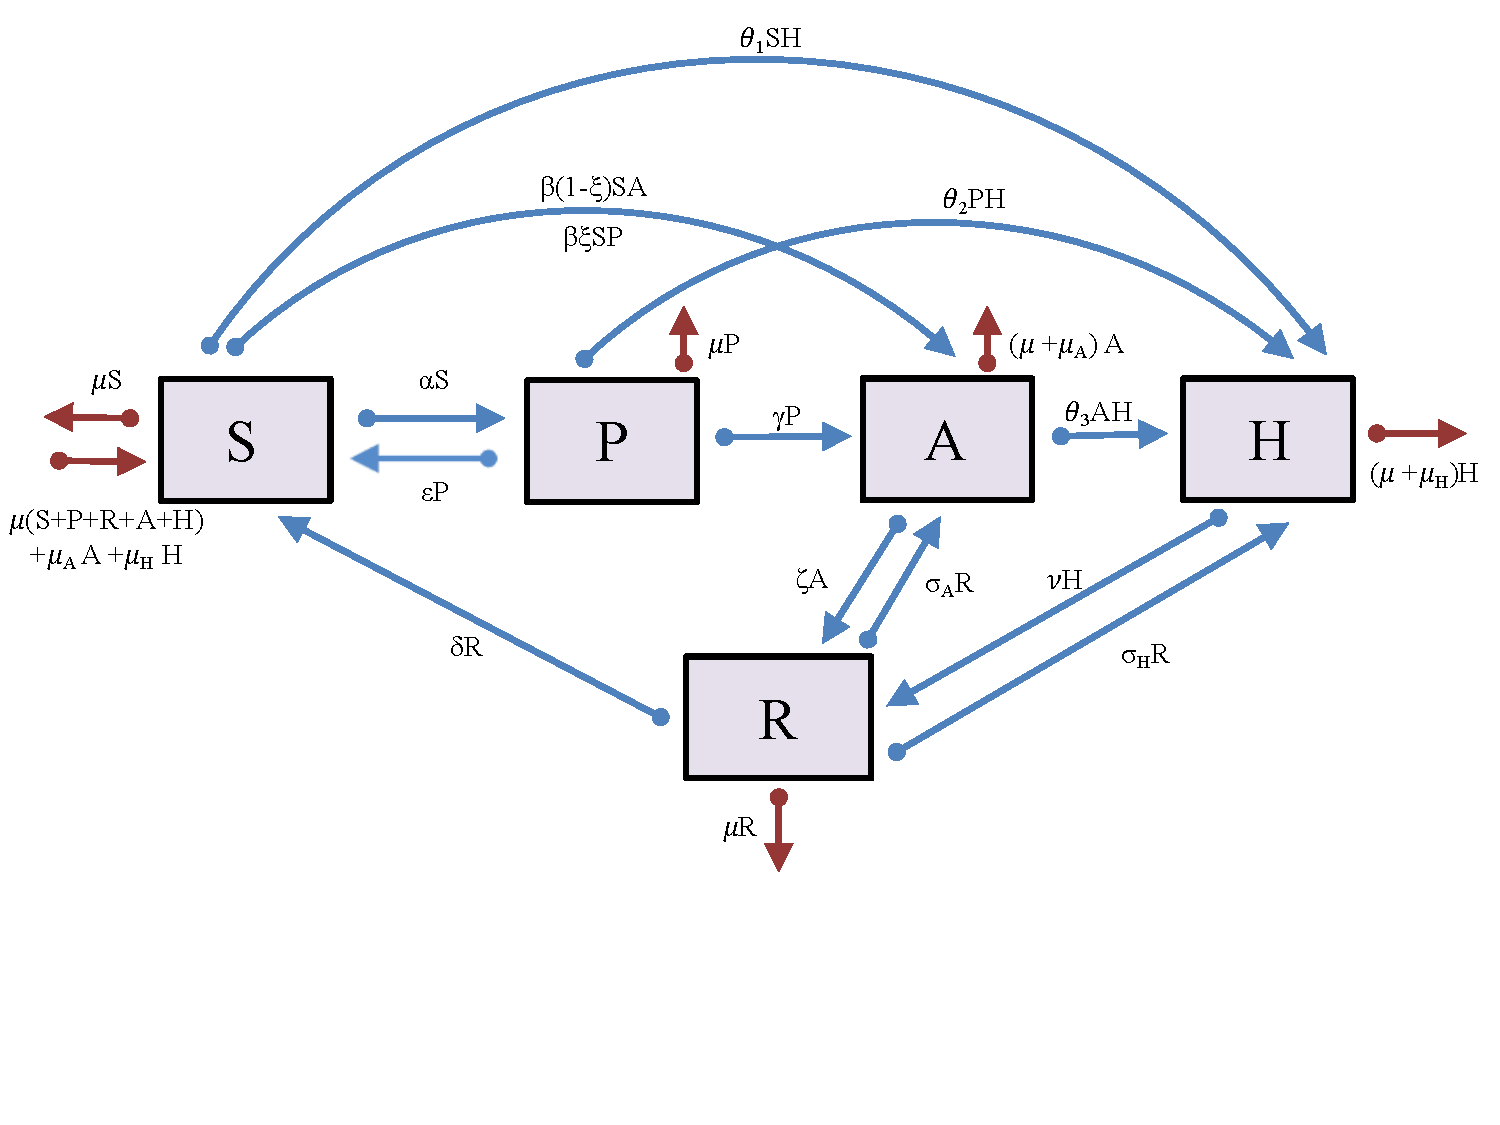
\includegraphics[scale=0.5]{heroin_schematic.pdf}
\vspace{-1cm}
\begin{center}
Figure 1: Flow chart for how individuals move among classes
\end{center} 

\textcolor{blue}{Assumptions we've made:} 

-The 5 compartments make up the entire population and the population is constant. \\
-Only considering addiction to opioids--not just any type of misuse. \\
-We take overdose to mean opioid overdose-related death. \\
-There is no permanent recovery class or immunity to addiction, so recovered individuals go back to the susceptible class. \\
-We do not know the history of the individuals, so they are a homogeneous group within each class (each individual will have the same probability of transitioning from one class to another, interacting with individuals from other classes, or dying). \\
*Note: we recognize there may be other possible pathways among the classes, but the ones we have chosen to include in our model are the ones we view as most important/realistic. 


\textcolor{blue}{Goals:}  
To address this apparent problem in today's society, we wish to: 

-Investigate the dynamics behind the opioid and heroin epidemic \\
-Identify important conditions relating to the reduction of opioid and heroin addicted individuals \\
-Explore management strategies for how to best treat pain with prescriptions while reducing opioid addiction and heroin use \\


 \textcolor{blue}{Data interested in:} 
We are interested in any type of data that is available from Knox County, including any of the following: 

-Proportions/percentages/total number of individuals in Knox County population who take prescription opioids, are addicted to opioids, are heroin users, or are in recovery (each month, year, etc.) \\
-Number of new opioid/heroin addictions per year in Knox county \\
-Overdose data (such as the number of addicted individuals or heroin users that died where the cause of death was overdose) \\ %broken into death/non-death or no? 
-Are individuals tracked to know the rate of transitioning from one class to another? \\
-Any other data that is available that may be pertinent to the heroin epidemic as a whole \\

\textcolor{blue}{Possible future extensions:}
We plan to add in more details in the future, but using this as a starting point for now. Examples of future work could include: 

-Looking into how gender, race, socioeconomic class, incarceration or geographical location play a role in susceptibility, drug use, recovery, etc. \\
-Breaking the recovery class into two different classes for opioid addicts and heroin users \\
-Effect of different treatments \\
-Significance of naloxone for reversing effects of overdoses \\


\pagebreak

%\bibliography{Knox_County_Public_Health_Summary}

 \end{document}
